\chapter{函数}
\section{函数}
\subsection{一元函数的概念}
\begin{definition}
设\(D\)是\(\mathbb{R}\)的一个非空子集,称映射\(f\colon D \to \mathbb{R}\)为定义在\(D\)上的一个\textbf{一元函数}(简称\textbf{函数}),通常记为\[
y = f(x), \qquad x \in D
\]其中点集\(D\)称为该函数的\textbf{定义域},\(x\)称为\textbf{自变量},\(y\)称为\textbf{因变量}.

函数定义中,对每个\(x \in D\),按对应法则\(f\),总有唯一确定的值\(y\)与之相应,%
这个值称为函数\(f\)在\(x\)处的\textbf{函数值},记作\(f(x)\),即\(y=f(x)\).
因变量\(y\)与自变量\(x\)之间的这种依赖关系,通常称为\textbf{函数关系}.
函数值\(f(x)\)的全体所构成的集合称为函数\(f\)的\textbf{值域},%
记作\(R_f\)或\(f(D)\),即\[
R_f = f(D) = \Set{ y \given y = f(x) \land x \in D }.
\]

函数的定义域通常按以下两种情形来确定:
一种是对有实际背景的函数,根据实际背景中变量的实际意义来确定.
另一种是对抽象地用算式表达的函数,通常约定这种函数的定义域是使得算式有意义的一切实数组成的集合,这种定义域称为函数的\textbf{自然定义域}.
\end{definition}

\begin{example}
函数\(y = \frac{1}{x}\)的自然定义域是\(\{ x \in \mathbb{R} \mid x \neq 0 \}\).
\end{example}

\begin{example}
函数\(y = \sqrt{x}\)的自然定义域是\(\{ x \in \mathbb{R} \mid x \geqslant 0 \}\).
\end{example}

\begin{definition}
如果给定一个对应法则,按这个法则,对每个\(x \in D\),总有确定但不唯一的\(y\)与之对应.
这样的不符合函数的定义的对应法则,习惯上称这种法则确定了一个\textbf{多值函数}.
对于多值函数,如果我们附加一些条件,使得在附加条件之下,按照这个法则,%
对每个\(x \in D\),总有唯一确定的实数值\(y\)与之对应,那么这就确定了一个函数.
我们称这样得到的函数为多值函数的\textbf{单值分支}.
\end{definition}

\subsection{多元函数的概念}
\begin{definition}
设\(D\)是\(\mathbb{R}^2\)的一个非空子集,称映射\(f\colon D \to \mathbb{R}\)为定义在\(D\)上的\textbf{二元函数},通常记为\[
z = f(x,y),
\quad \opair{x,y} \in D
\]或\[
z = f(P),
\quad P\opair{x,y} \in D
\]其中点集\(D\)称为该函数的\textbf{定义域},\(x\)、\(y\)称为\textbf{自变量},\(z\)称为\textbf{因变量}.
\end{definition}

\begin{definition}
类似地,设\(D\)是\(n\)维空间\(\mathbb{R}^n\)的一个非空子集,称映射\(f\colon D \to \mathbb{R}\)为定义在\(D\)上的\textbf{\(n\)元函数},通常记为\[
y = f(\v{x}{n}),
\quad \opair{\v{x}{n}} \in D
\]或简记为\[
y = f(\mat{x}),
\quad \mat{x}=\opair{\v{x}{n}} \in D
\]其中点集\(D\)称为该函数的\textbf{定义域},\(x\)、\(y\)称为\textbf{自变量},\(z\)称为\textbf{因变量}.
\end{definition}

\subsection{函数的性质}
\subsubsection{函数的有界性}
\begin{definition}
设函数\(f(x)\)的定义域为\(D\),数集\(X \subseteq D\).

如果存在数\(K_1\),使得\(f(x) \leqslant K_1\)对任一\(x \in X\)都成立,即\[
\forall x \in X, \exists K_1 \in \mathbb{R} \bigl[
	f(x) \leqslant K_1
\bigr],
\]则称函数\(f(x)\)在\(X\)上有\textbf{上界},而\(K_1\)称为函数\(f(x)\)在\(X\)上的一个上界.

如果存在数\(K_2\),使得\(f(x) \geqslant K_2\)对任一\(x \in X\)都成立,即\[
\forall x \in X, \exists K_2 \in \mathbb{R} \bigl[
	f(x) \geqslant K_2
\bigr],
\]则称函数\(f(x)\)在\(X\)上有\textbf{下界},而\(K_2\)称为函数\(f(x)\)在\(X\)上的一个下界.

如果存在正数\(M\),使得\(\abs{f(x)} \leqslant M\)对任一\(x \in X\)都成立,即\[
\forall x \in X, \exists K_2 \in \mathbb{R}^+ \bigl[
	\abs{f(x)} \leqslant M
\bigr],
\]则称函数\(f(x)\)在\(X\)上\textbf{有界}.
反之如果这样的\(M\)不存在,即\[
\exists x_0 \in X, \forall M > 0 \bigl[
	\abs{f(x_0)} > M
\bigr],
\]就称函数\(f(x)\)在\(X\)上\textbf{无界}.
\end{definition}

\begin{theorem}
设函数\(f(x)\)的定义域为\(D\),数集\(X \subseteq D\).
函数\(f(x)\)在\(X\)上有界的充要条件是它在\(X\)上既有上界又有下界.
\end{theorem}

\subsubsection{函数的单调性}
\begin{definition}
设函数\(f(x)\)的定义域为\(D\),区间\(I \subseteq D\).
如果对于区间\(I\)上任意两点\(x_1\)及\(x_2\),当\(x_1 < x_2\)时,恒有\[
f(x_1) < f(x_2),
\]则称函数\(f(x)\)在区间\(I\)上是\textbf{(严格)单调增加}的;
如果对于区间\(I\)上任意两点\(x_1\)及\(x_2\),当\(x_1 < x_2\)时,恒有\[
f(x_1) > f(x_2),
\]则称函数\(f(x)\)在区间\(I\)上是\textbf{(严格)单调减少}的.

单调增加的函数和单调减少的函数统称为\textbf{单调函数}.
\end{definition}

\subsubsection{函数的奇偶性}
\begin{definition}
设函数\(f(x)\)定义域为\(D=(-l,l)\)(\(l>0\)).
若对于任一\(x \in D\)都有\[
f(-x) = f(x),
\]恒成立,则称\(f(x)\)为\textbf{偶函数};
若对于任一\(x \in D\)都有\[
f(-x) = -f(x)
\]恒成立,则称\(f(x)\)为\textbf{奇函数}.
\end{definition}

\begin{property}
偶函数的图形是关于\(y\)轴对称的.
奇函数的图形是关于原点对称的.
\end{property}

\begin{property}
奇函数与奇函数之和、之差均为奇函数.
偶函数与偶函数之和、之差均为偶函数.
\begin{proof}
设\[
f(-x) = -f(x), \qquad g(-x) = -g(x).
\]令\(F(x) = f(x) \pm g(x)\),则\[
F(-x) = f(-x) \pm g(-x)
= [-f(x)] \pm [-g(x)]
= -[f(x) \pm g(x)]
= -F(x).
\qedhere
\]
\end{proof}
\end{property}

\begin{property}
奇函数与奇函数之积为偶函数.
\begin{proof}
设\[
f(-x) = -f(x), \qquad g(-x) = -g(x).
\]令\(F(x) = f(x) \cdot g(x)\),则\[
F(-x) = f(-x) \cdot g(-x)
= [-f(x)] \cdot [-g(x)]
= f(x) \cdot g(x)
= F(x).
\qedhere
\]
\end{proof}
\end{property}

\begin{property}
奇函数与偶函数之积为奇函数.
\begin{proof}
设\[
f(-x) = -f(x), \qquad g(-x) = g(x).
\]令\(F(x) = f(x) \cdot g(x)\),则\[
F(-x) = f(-x) \cdot g(-x)
= [-f(x)] \cdot g(x)
= - f(x) \cdot g(x)
= - F(x).
\qedhere
\]
\end{proof}
\end{property}

\begin{property}
偶函数与偶函数之积为偶函数.
\begin{proof}
设\[
f(-x) = f(x), \qquad g(-x) = g(x).
\]令\(F(x) = f(x) \cdot g(x)\),则\[
F(-x) = f(-x) \cdot g(-x) = f(x) \cdot g(x) = F(x).
\qedhere
\]
\end{proof}
\end{property}

\subsubsection{函数的周期性}
\begin{definition}
设函数\(f(x)\)的定义域为\(D\).
如果存在一个正数\(T\),使得对于任一\(x \in D\)有\((x + T) \in D\),且\[
f(x+ T) = f(x)
\]恒成立,则称\(f(x)\)为\textbf{周期函数},称\(T\)为\(f(x)\)的周期.

已知周期为\(T\)的函数.
如果对于任意数\(a \in (0,T)\)都有\[
f(x + a) \neq f(x),%
\]则称\(T\)为\textbf{最小正周期}.
\end{definition}

\begin{example}
狄利克雷(Dirichelet)函数\[
D(x) = \left\{ \begin{array}{ll}
1, & x \in \mathbb{Q}, \\
0, & x \in \mathbb{Q}^C.
\end{array} \right.
\]是一个周期函数,任何正有理数\(r\)都是它的周期.因为不存在最小的正有理数,所以它没有最小正周期.
\end{example}

\section{反函数与复合函数}
\begin{definition}[反函数]
设函数\(f\colon D \to f(D)\)是单射,则它存在逆映射\(f^{-1}: f(D) \to D\),称此映射\(f^{-1}\)为函数\(f\)的\textbf{反函数}.
相对于反函数\(y=f^{-1}(x)\)来说,原来的函数\(y=f(x)\)称为\textbf{直接函数}.
\end{definition}

\begin{property}
将直接函数\(y=f(x)\)和它的反函数\(y=f^{-1}(x)\)的图形画在同一坐标平面上,%
这两个图形关于直线\(y=x\)是对称的.
\end{property}

\begin{definition}
设函数\(y=f(u)\)的定义域为\(D_f\),函数\(u=g(x)\)的定义域为\(D_g\),且其值域\(R_g \subseteq D_f\),则函数\[
y = f[g(x)],
\quad x \in D_g
\]称为由函数\(u=g(x)\)与函数\(y=f(u)\)构成的\textbf{复合函数},它的定义域为\(D_g\),变量\(u\)称为\textbf{中间变量}.

函数\(g\)与函数\(f\)构成的复合函数,即按“先\(g\)后\(f\)”的次序复合的函数,通常记为\(f \circ g\),即\[
(f \circ g)(x) = f[g(x)].
\]
\end{definition}

\begin{example}
设函数\(f(x)\)的定义域为\((-l,l)\),试证:在\((-l,l)\)上必存在偶函数\(g(x)\)和奇函数\(h(x)\),使得\[
f(x) = g(x)+h(x).
\]
\begin{proof}
首先假设这样的\(g(x)\)、\(h(x)\)存在,即\[
f(x) = g(x) + h(x),
\]\[
g(-x) = g(x),
\]\[
h(-x) = -h(x).
\]于是有\[
f(-x) = g(-x) + h(-x) = g(x) - h(x).
\]

由此可知,只需要取\[
g(x) = \frac{1}{2} [f(x) + f(-x)],
\]\[
h(x) = \frac{1}{2} [f(x) - f(-x)]
\]即可满足题设要求.
\end{proof}
\end{example}

\section{常见函数}
\subsection{绝对值函数}
\begin{definition}[绝对值]
设\(x \in \mathbb{R}\),则称函数\[
f(x) = \left\{ \begin{array}{c}
x, \quad x \geqslant 0 \\
-x, \quad x < 0
\end{array} \right.
\]为\(x\)的绝对值,记作\(\abs{x}\).
\end{definition}

\begin{figure}[ht]
\centering
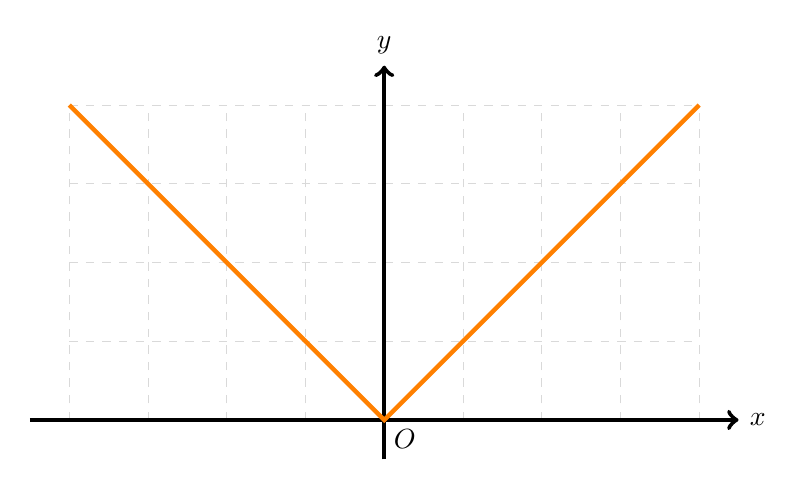
\begin{tikzpicture}
	\draw[help lines, color=gray!30, dashed] (-4,0) grid (4,4);
	\draw[->, ultra thick] (-4.5,0) -- (4.5,0) node[right]{\(x\)};
	\draw[->, ultra thick] (0,-0.5) -- (0,4.5) node[above]{\(y\)};
	\draw (0,0)node[below right]{\(O\)};
	\draw[orange,ultra thick] (-4,4)--(0,0)--(4,4);
\end{tikzpicture}
\caption{绝对值函数\(\abs{x}\)的图形}
\end{figure}

\subsection{符号函数}
\begin{definition}[符号函数]
函数\[
f(x) = \left\{ \begin{array}{cc}
1, & x > 0 \\
0, & x = 0 \\
-1, & x < 0 \\
\end{array} \right.
\]称为\textbf{符号函数},记作\(\sgn x\).
\end{definition}

\begin{figure}[ht]
\centering
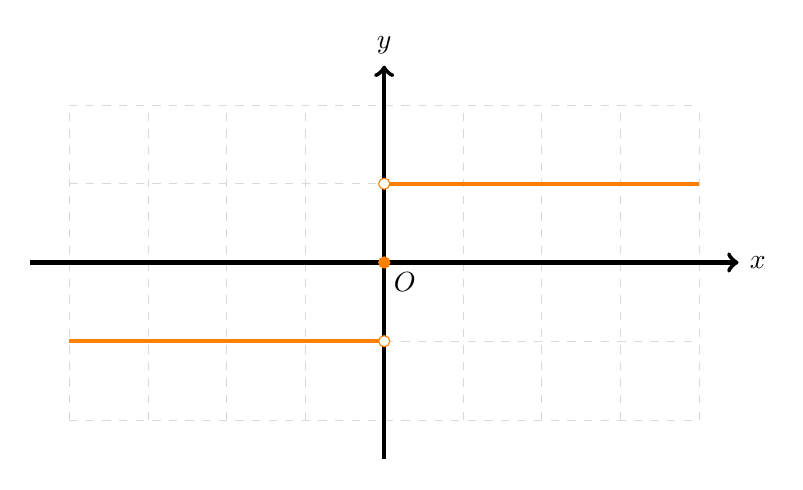
\begin{tikzpicture}
	\draw[help lines, color=gray!30, dashed] (-4,-2) grid (4,2);
	\draw[->, ultra thick] (-4.5,0) -- (4.5,0) node[right]{\(x\)};
	\draw[->, ultra thick] (0,-2.5) -- (0,2.5) node[above]{\(y\)};
	\draw (0,0)node[below right]{\(O\)};
	\draw[orange,ultra thick] (-4,-1)--(0,-1) (0,1)--(4,1);
	\draw[draw=orange,fill=orange] (0,0)circle(2pt);
	\draw[draw=orange,fill=white] (0,1)circle(2pt) (0,-1)circle(2pt);
\end{tikzpicture}
\caption{符号函数\(\sgn x\)的图形}
\end{figure}

\subsection{取整函数}
\begin{definition}[取整函数]
设\(x \in \mathbb{R}\),定义:
\begin{enumerate}
\item 向下取整函数\(\floor{x}\)为不大于\(x\)的最大整数;
\item 向上取整函数\(\ceil{x}\)为不小于\(x\)的最小整数.
\end{enumerate}
在未特别说明的情况下,取整函数\([x]\)是指向下取整函数,即\[
[x] = \floor{x}.
\]
\end{definition}

\begin{figure}
\def\subwidth{.45\linewidth}
\def\subscale{.9}
\begin{subfigure}[b]{\subwidth}%
\centering
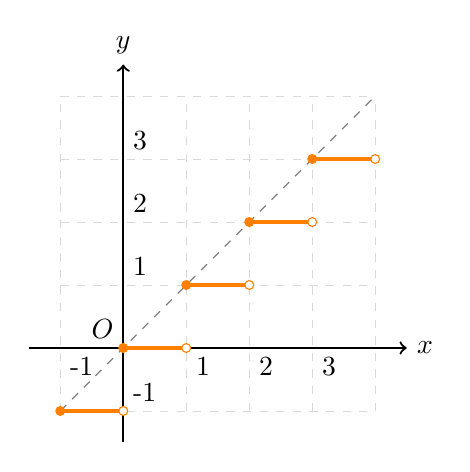
\begin{tikzpicture}[scale=\subscale]
	\tikzstyle{sx}=[draw=orange,fill=orange]
	\tikzstyle{kx}=[draw=orange,fill=white]
	\draw[help lines, color=gray!30, dashed] (-1,-1) grid (4,4);
	\draw[dashed, color=gray] (-1,-1) -- (4,4);
	\draw[->, thick] (-1.5,0) -- (4.5,0) node[right]{\(x\)};
	\draw[->, thick] (0,-1.5) -- (0,4.5) node[above]{\(y\)};
	\foreach \i in {-1,...,3} {
		\draw[ultra thick,orange] (\i,\i)--(\i+1,\i);
		\fill[sx] (\i,\i)circle(2pt);
		\fill[kx] (\i+1,\i)circle(2pt);
		\ifnum\i=0\relax\else
			\draw(\i,0)node[below right]{\i};
			\draw(0,\i)node[above right]{\i};
		\fi;
	}
	\draw (0,0)node[above left]{\(O\)};
\end{tikzpicture}
\subcaption{向下取整函数\(\floor{x}\)}
\end{subfigure}
\begin{subfigure}[b]{\subwidth}%
\centering
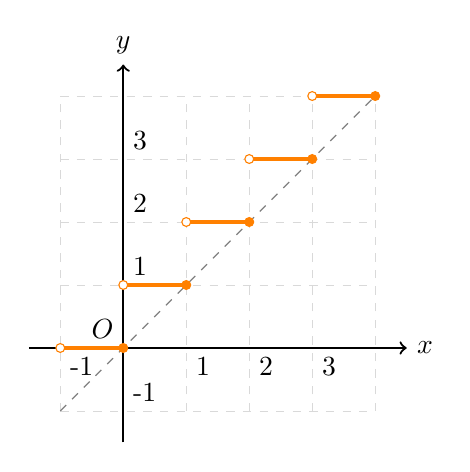
\begin{tikzpicture}[scale=\subscale]
	\tikzstyle{sx}=[draw=orange,fill=orange]
	\tikzstyle{kx}=[draw=orange,fill=white]
	\draw[help lines, color=gray!30, dashed] (-1,-1) grid (4,4);
	\draw[dashed, color=gray] (-1,-1) -- (4,4);
	\draw[->, thick] (-1.5,0) -- (4.5,0) node[right]{\(x\)};
	\draw[->, thick] (0,-1.5) -- (0,4.5) node[above]{\(y\)};
	\foreach \i in {-1,...,3} {
		\draw[ultra thick,orange] (\i,\i+1)--(\i+1,\i+1);
		\fill[kx] (\i,\i+1)circle(2pt);
		\fill[sx] (\i+1,\i+1)circle(2pt);
		\ifnum\i=0\relax\else
			\draw(\i,0)node[below right]{\i};
			\draw(0,\i)node[above right]{\i};
		\fi;
	}
	\draw (0,0)node[above left]{\(O\)};
\end{tikzpicture}
\subcaption{向上取整函数\(\ceil{x}\)}
\end{subfigure}
\caption{取整函数的图形}
\end{figure}

\begin{property}
一般地,对于\(x\in\mathbb{R}\),总有\begin{equation}
x - 1 < \floor{x} \leqslant x \leqslant \ceil{x} < x + 1.
\end{equation}
\end{property}

\begin{property}
对于\(x\in\mathbb{Z}\),总有\begin{equation}
\ceil{n/2} + \floor{n/2} = n.
\end{equation}
\end{property}

\begin{property}
对于任意实数\(x \geqslant 0\)和整数\(a,b>0\),总有\begin{gather}
\ceil*{\frac{\ceil{x/a}}{b}} = \ceil*{\frac{x}{ab}}, \\
\floor*{\frac{\floor{x/a}}{b}} = \floor*{\frac{x}{ab}}, \\
\ceil*{\frac{a}{b}} \leqslant \frac{a+(b-1)}{b}, \\
\floor*{\frac{a}{b}} \geqslant \frac{a-(b-1)}{b}.
\end{gather}
\end{property}

\subsection{单位阶跃函数}
\begin{definition}
函数\[
f(x) = \left\{ \begin{array}{cc}
0, & x < 0, \\
1, & x \geqslant 1
\end{array} \right.
\]称为\DefineConcept{单位阶跃函数}(或称为\DefineConcept{赫维赛德(Heaviside)阶跃函数}).
\end{definition}

\begin{figure}[h!]
\centering
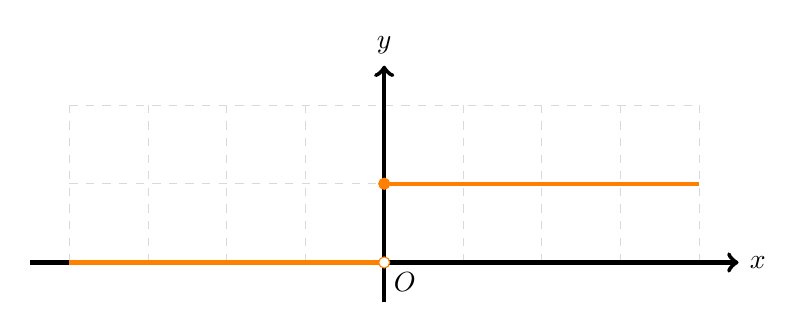
\begin{tikzpicture}
	\draw[help lines, color=gray!30, dashed] (-4,0) grid (4,2);
	\draw[->, ultra thick] (-4.5,0) -- (4.5,0) node[right]{\(x\)};
	\draw[->, ultra thick] (0,-.5) -- (0,2.5) node[above]{\(y\)};
	\draw (0,0)node[below right]{\(O\)};
	\draw[orange,ultra thick] (-4,0)--(0,0) (0,1)--(4,1);
	\draw[draw=orange,fill=orange] (0,1)circle(2pt);
	\draw[draw=orange,fill=white] (0,0)circle(2pt);
\end{tikzpicture}
\caption{单位阶跃函数的图形}
\end{figure}

\subsection{幂函数、指数函数、对数函数}
\begin{definition}
同一个数\(a\)(\(a\in\mathbb{R}\))连续相乘\(b\)(\(b\in\mathbb{N}\))次所得的乘积称作“\(a\)的\(b\)次方”(或“\(a\)的\(b\)次幂”),记作\(a^b\),即\[
a^b = \underbrace{a \times a \times \dotsm \times a}_{b\text{次}} = \prod\limits_{i=1}^b a.
\]

特别地,规定:\(a^0 = 1\),\(a^{-n} = \frac{1}{a^n}\),其中\(a\in\mathbb{R}^*\),\(n\in\mathbb{N}^+\).
\end{definition}

\begin{figure}[ht]
\centering
\begin{tikzpicture}
\def\r{\textcolor{orange}}
\def\b{\textcolor{blue}}
\def\p{\textcolor{purple}}
\draw (0,0)node{\(\r{a}^{\b{b}} = \p{c} \iff \log_{\r{a}} \p{c} = \b{b}\)};
\draw (-2.2,-.5)node{\r{底数}}
	(-2.2,.5)node{\b{指数}}
	(-1,-.5)node{\p{幂}}
	(.3,-.5)node{\r{底数}}
	(1.4,-.5)node{\p{真数}}
	(2.3,.5)node{\b{对数}};
\draw[->] (-1.7,-.3)--(-1.7,-1)--(.84,-1)->(.84,-.3); %a
\draw[->] (-1.55,.3)--(-1.55,1)--(1.7,1)->(1.7,.3); %b
\draw[->] (-.86,.3)--(-.86,.7)--(1.1,.7)->(1.1,.3); %c
\end{tikzpicture}
\caption{底数、指数、幂与对数的联系}
\label{figure:函数.底数、指数、幂与对数的联系}
\end{figure}

\subsubsection{幂函数的概念}
\begin{definition}[幂函数]
形如\(y=x^{\mu}\)(\(\mu \in \mathbb{R}\))的函数,称为\textbf{幂函数}.
\end{definition}

\subsubsection{幂函数的性质}
\begin{property}
幂函数具有以下性质:
\begin{enumerate}
\item 当\(\mu = 0\)时,幂函数\(y=x^{\mu}=1\)是常数函数;
\item 当\(\mu\)为正奇数时,幂函数\(y=x^{\mu}\)为奇函数,其定义域、值域均为\((-\infty,+\infty)\),它在定义域内恒单调递增;
\item 当\(\mu\)为正偶数时,幂函数\(y=x^{\mu}\)为偶函数,其定义域为\((-\infty,+\infty)\),其值域为\([0,+\infty)\),它在\((-\infty,0]\)上单调递减,在\([0,+\infty)\)上单调递增;
\item 当\(\mu\)为负奇数时,幂函数\(y=x^{\mu}\)又称\textbf{比例函数}(%
若幂函数前有常系数大于零则称之为\textbf{正比例函数},%
% Plot[Evaluate[x^-n /. n -> {1, 2, 3, 4, 5}], {x, 0, 2}, PlotRange -> {0, 2}, PlotLegends -> Automatic]
若幂函数前有常系数小于零则称之为\textbf{反比例函数}),%
% Plot[Evaluate[x^-n /. n -> {1, 2, 3, 4, 5}], {x, -2, 0}, PlotRange -> {-2, 2}, PlotLegends -> Automatic]
其定义域、值域为\((-\infty,0)\cup(0,+\infty)\),它在区间\((-\infty,0)\)和\((0,+\infty)\)内单调递减;
\item 当\(\mu\)为负偶数时,幂函数\(y=x^{\mu}\)为偶函数,其定义域为\((-\infty,0)\cup(0,+\infty)\),其值域为\((0,+\infty)\),它在\((-\infty,0)\)内单调递增,在\((0,+\infty)\)内单调递减;
\item 当\(\mu = \frac{m}{n} \in \mathbb{Q}\)(\(m\)、\(n\)是互质的整数)时,幂函数\(y=x^{\mu}=x^{\frac{m}{n}}\)可改写为\(y=\sqrt[n]{x^m}\)(\(\mu>0\)时)或\(y=\frac{1}{\sqrt[n]{x^m}}\)(\(\mu<0\)时).
\end{enumerate}
\end{property}

\subsubsection{指数函数的概念}
\begin{definition}[指数函数]
形如\(y=a^x\)(\(a>0 \land a \neq 1\))的函数,称为以\(a\)为底的\textbf{指数函数}.
将\(a\)(\(a \neq 0\))的倒数\(\frac{1}{a}\)记作\(a^{-1}\).
将\(a\)(\(a \geqslant 0\))的\(x\)次方根\(\sqrt[x]{a}\)记作\(a^{\frac{1}{x}}\).
规定任一实数的1次幂为该实数本身,即\(a^1=a\).
规定任一非零实数的零次幂为1,即\(a^0=1\).
\end{definition}

\subsubsection{对数函数的概念}
\begin{definition}[对数函数]
形如\(y=\log_a x\)(\(a>0 \land a \neq 1\))的函数,称为以\(a\)为底的\textbf{对数函数}.

特别地,以\(10\)为底的对数称为\textbf{常用对数},记作\(y = \lg x\);以常数\(e\)为底的对数称为\textbf{自然对数},记作\(y = \ln x\).
\end{definition}

\subsubsection{指数函数、对数函数的性质}
\begin{property}
指数函数\(y = a^x\)与对数函数\(y = \log_a x\)互为反函数,即\[
a^{\log_a x} = x, \qquad \log_a a^x = x.
\]它们具有以下性质:
\begin{center}
\def\arraystretch{1.5}
\begin{tabular}{|*{2}{p{5cm}|}}
\hline
\(a^x a^y = a^{x+y}\) & \(\log_a xy = \log_a x + \log_a y\) \\ \hline
\(\frac{a^x}{a^y} = a^{x-y}\) & \(\log_a \frac{x}{y} = \log_a x - \log_a y\) \\ \hline
\((a^x)^y = a^{xy}\) & \(\log_a x^y = y \log_a x\) \\ \hline
\end{tabular}
\end{center}
\end{property}

\begin{theorem}[换底公式]
一般地,\[
\log_a b = \frac{\log_c b}{\log_c a},
\]其中\(a,c\in(0,1)\cup(1,+\infty)\),\(b\in(0,+\infty)\).

特殊地,\[
\log_a b = \frac{1}{\log_b a},
\]其中\(a,b\in(0,1)\cup(1,+\infty)\).
\end{theorem}

\begin{corollary}
若\(a,a^x \in (0,1)\cup(1,+\infty)\),则\[
\log_{a^x} b^y = \frac{y}{x} \log_a b.
\]
\end{corollary}

\begin{example}
证明:\begin{equation}\label{equation:函数.真底互换公式}
a^{\ln b} = b^{\ln a}.
\end{equation}
\begin{proof}
在\cref{equation:函数.真底互换公式} 等号左右变量分别取对数,得\[
\ln(a^{\ln b}) = \ln b \ln a, \qquad
\ln(b^{\ln a}) = \ln a \ln b,
\]显然两者相等,故\(a^{\ln b} = b^{\ln a}\)成立.
\end{proof}
\end{example}

\subsection{三角函数}
\subsubsection{三角函数的概念}
\begin{definition}
如图所示,\(\angle{BAC} = \theta\),\(\angle{ABC} = \frac{\pi}{2}\).
\begin{center}
\begin{tikzpicture}
\draw[help lines, color=gray!30, dashed] (0,0) grid (4,3);
\coordinate (A) at (0,0);
\coordinate (B) at (4,0);
\coordinate (C) at (4,3);
\draw (A)node[left]{\(A\)} -- (B)node[right]{\(B\)}node[midway,below]{\(c\)} -- (C)node[right]{\(C\)}node[midway,right]{\(a\)} -- (A)node[midway,left,above]{\(b\)} pic["\(\theta\)",draw=orange,-,angle eccentricity=2,angle radius=0.3cm]{angle=B--A--C} pic[draw=gray,-,angle radius=0.3cm]{right angle=C--B--A};
\end{tikzpicture}
\end{center}

定义三角函数如下:
\begin{center}
\def\arraystretch{1.5}
\begin{tabular}{|c|c|l|}
\hline
名称 & 解析式 & 定义域 \\ \hline
正弦 & \(\sin \theta = a/b\) & \(-\infty < \theta < +\infty\) \\ \hline
余弦 & \(\cos \theta = c/b\) & \(-\infty < \theta < +\infty\) \\ \hline
正切 & \(\tan \theta = a/c\) & \(\theta\neq k\pi+\frac{\pi}{2}\ (k\in\mathbb{Z})\) \\ \hline
余切 & \(\cot \theta = c/a\) & \(\theta\neq k\pi\ (k\in\mathbb{Z})\) \\ \hline
正割 & \(\sec \theta = b/c\) & \(\theta\neq k\pi+\frac{\pi}{2}\ (k\in\mathbb{Z})\) \\ \hline
余割 & \(\csc \theta = b/a\) & \(\theta\neq k\pi\ (k\in\mathbb{Z})\) \\ \hline
\end{tabular}
\end{center}
\end{definition}

\begin{example}
下面列出一些特殊的正弦函数值:\[
\sin0 = 0, \quad
\sin\frac{\pi}{6} = \frac{1}{2}, \quad
\sin\frac{\pi}{4} = \frac{\sqrt{2}}{2}, \quad
\sin\frac{\pi}{3} = \frac{\sqrt{3}}{2},
\]\[
\sin\frac{\pi}{2} = 1, \quad
\sin\pi = 0, \quad
\sin\frac{3\pi}{2} = -1.
\]

\begin{figure}[ht]
\centering
\begin{tikzpicture}
\pgfmathsetmacro{\r}{2}
\pgfmathsetmacro{\ax}{\r*cos(30)}
\pgfmathsetmacro{\ay}{\r*sin(30)}
\pgfmathsetmacro{\b}{\r/sqrt(2)}
\coordinate (O)at(0,0);
\draw(O)circle(\r);
\begin{scope}[dashed,color=gray!50,text=black]
\draw(O)--(\r,0)node[left]{\(0\)}node[right]{\(0\)}
(O)--(\ax,\ay)node[below left]{\(\tfrac{\pi}{6}\)}node[right]{\(\tfrac{1}{2}\)}
(O)--(\b,\b)node[below left]{\(\tfrac{\pi}{4}\)}node[above right]{\(\tfrac{\sqrt2}{2}\)}
(O)--(\ay,\ax)node[below left]{\(\tfrac{\pi}{3}\)}node[above]{\(\tfrac{\sqrt3}{2}\)}
(O)--(0,\r)node[below]{\(\tfrac{\pi}{2}\)}node[above]{\(1\)}
(O)--(-\ay,\ax)node[below right]{\(\tfrac{2\pi}{3}\)}node[above]{\(\tfrac{\sqrt3}{2}\)}
(O)--(-\b,\b)node[below right]{\(\tfrac{3\pi}{4}\)}node[above left]{\(\tfrac{\sqrt2}{2}\)}
(O)--(-\ax,\ay)node[below right]{\(\tfrac{5\pi}{6}\)}node[left]{\(\tfrac{1}{2}\)}
(O)--(-\r,0)node[right]{\(\pi\)}node[left]{\(0\)}
(O)--(-\ax,-\ay)node[above right]{\(\tfrac{7\pi}{6}\)}node[left]{\(-\tfrac{1}{2}\)}
(O)--(-\b,-\b)node[above right]{\(\tfrac{5\pi}{4}\)}node[below left]{\(-\tfrac{\sqrt2}{2}\)}
(O)--(-\ay,-\ax)node[above right]{\(\tfrac{4\pi}{3}\)}node[below]{\(-\tfrac{\sqrt3}{2}\)}
(O)--(0,-\r)node[above]{\(\tfrac{3\pi}{2}\)}node[below]{\(-1\)}
(O)--(\ay,-\ax)node[above left]{\(\tfrac{5\pi}{3}\)}node[below]{\(-\tfrac{\sqrt3}{2}\)}
(O)--(\b,-\b)node[above left]{\(\tfrac{7\pi}{4}\)}node[below right]{\(-\tfrac{\sqrt2}{2}\)}
(O)--(\ax,-\ay)node[above left]{\(\tfrac{11\pi}{6}\)}node[right]{\(-\tfrac{1}{2}\)}
;
\end{scope}
\begin{scope}[very thick,->]
\draw(-1,0)--(1,0)node[above left]{\(x\)};
\draw(0,-1)--(0,1)node[below right]{\(y\)};
\end{scope}
\end{tikzpicture}
\caption{正弦函数\(\sin x\)的辅助圆与特殊值}
\end{figure}

特殊的余弦函数值:\[
\cos0 = 1, \quad
\cos\frac{\pi}{6} = \frac{\sqrt{3}}{2}, \quad
\cos\frac{\pi}{4} = \frac{\sqrt{2}}{2}, \quad
\cos\frac{\pi}{3} = \frac{1}{2},
\]\[
\cos\frac{\pi}{2} = 0, \quad
\cos\pi = -1, \quad
\cos\frac{3\pi}{2} = 0.
\]
\end{example}

\subsubsection{三角函数的性质}
\begin{property}
根据三角函数的定义,显然有\begin{gather}
\cot\theta = \frac{1}{\tan\theta}, \\
\sec\theta = \frac{1}{\cos\theta}, \\
\csc\theta = \frac{1}{\sin\theta}.
\end{gather}
\end{property}

\begin{theorem}[毕达哥拉斯三角恒等式]
\begin{figure}
\def\subwidth{.5\linewidth}
\def\subscale{.8}
    \begin{subfigure}[b]{\subwidth}%
    \centering
    \begin{tikzpicture}[scale=\subscale]
        \draw[help lines, color=gray!30, dashed] (0,0) grid (4,3);
        \coordinate (A) at (0,0);
        \coordinate (B) at (4,0);
        \coordinate (C) at (4,3);
        \draw (A)node[left]{\(A\)} -- (B)node[right]{\(B\)}node[midway,below]{\(\cos\theta\)} -- (C)node[right]{\(C\)}node[midway,right]{\(\sin\theta\)} -- (A)node[midway,above left]{\(1\)} pic["\(\theta\)",draw=orange,-,angle eccentricity=2,angle radius=0.3cm]{angle=B--A--C} pic[draw=gray,-,angle radius=0.3cm]{right angle=C--B--A};
    \end{tikzpicture}
    \subcaption{正弦、余弦辅助三角形}
    \end{subfigure}%
    \begin{subfigure}[b]{\subwidth}%
    \centering
    \begin{tikzpicture}[scale=\subscale]
        \draw[help lines, color=gray!30, dashed] (0,0) grid (4,3);
        \coordinate (A) at (0,0);
        \coordinate (B) at (4,0);
        \coordinate (C) at (4,3);
        \draw (A)node[left]{\(A\)} -- (B)node[right]{\(B\)}node[midway,below]{\(1\)} -- (C)node[right]{\(C\)}node[midway,right]{\(\tan\theta\)} -- (A)node[midway,above left]{\(\sec\theta\)} pic["\(\theta\)",draw=orange,-,angle eccentricity=2,angle radius=0.3cm]{angle=B--A--C} pic[draw=gray,-,angle radius=0.3cm]{right angle=C--B--A};
    \end{tikzpicture}
    \subcaption{正切、正割辅助三角形}
    \end{subfigure}%
\caption{两种特殊的辅助三角形}
\label{figure:函数.两种特殊的辅助三角形}
\end{figure}

结合\cref{figure:函数.两种特殊的辅助三角形} ,根据勾股定理可得
\begin{gather}
\sin^2 \theta + \cos^2 \theta = 1, \\
\tan^2 \theta + 1 = \sec^2 \theta, \\
1 + \cot^2 \theta = \csc^2 \theta.
\end{gather}
\end{theorem}

\begin{property}
%sine
\begin{figure}
\centering
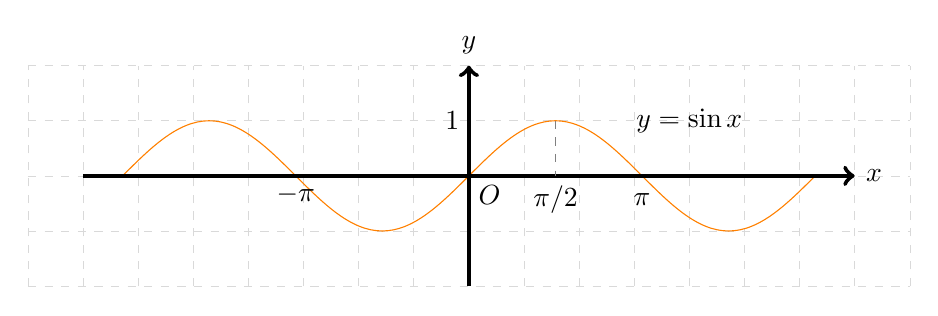
\begin{tikzpicture}[scale=0.7]
	\draw[help lines, color=gray!30, dashed] (-8,-2) grid (8,2);
	\draw[color=orange] (-2*pi,0) sin (-1.5*pi,1) cos (-pi,0) sin (-0.5*pi,-1) cos (0,0) sin (0.5*pi,1) cos (pi,0) sin (1.5*pi,-1) cos (2*pi,0);

	\draw[->, ultra thick] (-7,0) -- (7,0) node[right]{\(x\)};
	\draw[->, ultra thick] (0,-2) -- (0,2) node[above]{\(y\)};
	\draw (0.5*pi,0)node[below]{\(\pi/2\)};
	\draw[dashed, color=gray] (0.5*pi,1) -- (0.5*pi,0);
	\draw (0,0)node[below right]{\(O\)}
		(0,1)node[left]{\(1\)}
		(pi,0)node[below=3pt]{\(\pi\)}
		(-pi,0)node[below]{\(-\pi\)}
		(4,1)node{\(y=\sin x\)};
\end{tikzpicture}
\caption{正弦函数的图形}
\label{figure:函数.正弦函数的图形}
\end{figure}

如\cref{figure:函数.正弦函数的图形} ,可以观察得出正弦函数的若干性质.
正弦函数是周期函数,其周期为\(T = 2\pi\).
正弦函数在区间\([2k\pi-\frac{\pi}{2},2k\pi+\frac{\pi}{2})\)上单调递增;
在区间\([2k\pi+\frac{\pi}{2},2k\pi+\frac{3\pi}{2})\)上单调递增;
当\(x=\frac{\pi}{2}+2k\pi\)时取得极大值\(1\);
当\(x=\frac{3\pi}{2}+2k\pi\)时,正弦函数取得极小值\(-1\)(\(k\in\mathbb{Z}\)).
正弦函数是奇函数,其图形关于坐标原点\(O\)中心对称,即满足\(\sin(-x)=-\sin x\).
\end{property}

\begin{property}
%cosine
\begin{figure}
\centering
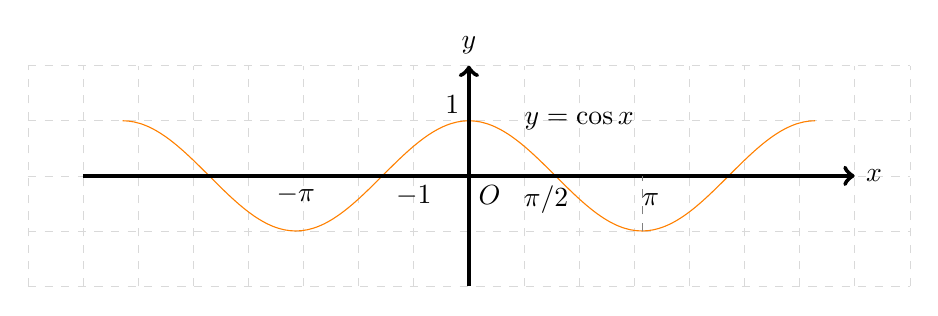
\begin{tikzpicture}[scale=0.7]
	\draw[help lines, color=gray!30, dashed] (-8,-2) grid (8,2);
	\draw[color=orange] (-2*pi,1) cos (-1.5*pi,0) sin (-pi,-1) cos (-0.5*pi,0) sin (0,1) cos (0.5*pi,0) sin (pi,-1) cos (1.5*pi,0) sin (2*pi,1);

	\draw[->, ultra thick] (-7,0) -- (7,0) node[right]{\(x\)};
	\draw[->, ultra thick] (0,-2) -- (0,2) node[above]{\(y\)};
	\draw (1.4,0)node[below]{\(\pi/2\)};
	\draw[dashed, color=gray] (pi,-1) -- (pi,0);
	\draw (0,0)node[below right]{\(O\)}
		(-1,0)node[below]{\(-1\)}
		(0,1.3)node[left]{\(1\)}
		(3.3,0)node[below=3pt]{\(\pi\)}
		(-pi,0)node[below]{\(-\pi\)}
		(2,1)node{\(y=\cos x\)};
\end{tikzpicture}
\caption{余弦函数的图形}
\label{figure:函数.余弦函数的图形}
\end{figure}

如\cref{figure:函数.余弦函数的图形} ,可以观察得出余弦函数的若干性质.
余弦函数也是周期函数,其周期为\(T = 2\pi\).
余弦函数在区间\([2k\pi,\pi+2k\pi)\)上单调递减;
在区间\([\pi+2k\pi,2\pi+2k\pi)\)上单调递增;
当\(x=2k\pi\)时取得极大值\(1\);
当\(x=(2k-1)\pi\)时取得极小值\(-1\)(\(k\in\mathbb{Z}\)).
余弦函数是偶函数,其图形关于\(y\)轴对称,即满足\(\cos(-x)=\cos x\).
\end{property}

\begin{property}
%tangent
\begin{figure}
\centering
\begin{tikzpicture}
\draw[help lines, color=gray!30, dashed] (-6,-4) grid (6,4);

\foreach \idx in {-1,0,1,2}{
	\pgfmathsetmacro{\start}{\idx*pi-1.3};
	\pgfmathsetmacro{\left}{(\idx-0.5)*pi};
	\pgfmathsetmacro{\end}{\idx*pi+1.3};
	\draw[dashed,red] (\left,-4) -- (\left,4);
	\ifthenelse{\equal{2}{\idx}} {} {
		\draw[color=orange] plot[domain=\start:\end, samples=100] (\x, {tan(\x r)})
	};
}

\draw [->, ultra thick] (-6,0) -- (6,0) node[right]{\(x\)};
\draw [->, ultra thick] (0,-4) -- (0,4) node[above]{\(y\)};
\draw node[] at(1.4,-0.5) {\(\frac{\pi}{2}\)};
\draw node[] at(0.3,-0.3) {\(O\)}
		node[] at(-0.3,1) {\(1\)}
		node[] at(3.14159,-0.5) {\(\pi\)}
		node[] at(-3.14159,-0.5) {\(-\pi\)}
		node[] at(2,1) {\(y=\tan x\)};
\end{tikzpicture}
\caption{正切函数的图形}
\label{figure:函数.正切函数的图形}
\end{figure}

如\cref{figure:函数.正切函数的图形} ,可以观察得出正切函数的若干性质.
正切函数是周期函数,其周期为\(T = \pi\).
正切函数在区间\((k\pi-\frac{\pi}{2},k\pi+\frac{\pi}{2})\)(\(k\in\mathbb{Z}\))上单调递增.
正切函数是奇函数,其图形关于坐标原点\(O\)中心对称,即满足\(\tan(-x)=-\tan x\).
\end{property}

\subsubsection{和积互化公式}
\begin{theorem}[和积互化公式]
\begin{align}
\sin(\alpha\pm\beta) &= \sin\alpha\cos\beta\pm\cos\alpha\sin\beta, \label{equation:函数.三角函数.和积互化公式1} \\
\cos(\alpha\pm\beta) &= \cos\alpha\cos\beta\mp\sin\alpha\sin\beta, \label{equation:函数.三角函数.和积互化公式2} \\
\tan(\alpha\pm\beta) &= \frac{\tan\alpha\pm\tan\beta}{1\mp\tan\alpha\tan\beta}, \label{equation:函数.三角函数.和积互化公式3} \\
\cot(\alpha\pm\beta) &= \frac{\cot\alpha\cot\beta\mp 1}{\cot\beta\pm\cot\alpha}, \label{equation:函数.三角函数.和积互化公式4} \\
\sec(\alpha\pm\beta) &= \frac{\sec\alpha\sec\beta}{1\mp\tan\alpha\tan\beta}, \label{equation:函数.三角函数.和积互化公式5} \\
\csc(\alpha\pm\beta) &= \frac{\csc\alpha\csc\beta}{\cot\beta\pm\cot\alpha}, \label{equation:函数.三角函数.和积互化公式6} \\
\sin \alpha \cos \beta &= \frac{\sin (\alpha + \beta) + \sin (\alpha - \beta)}{2}, \label{equation:函数.三角函数.和积互化公式7} \\
\cos \alpha \sin \beta &= \frac{\sin (\alpha + \beta) - \sin (\alpha - \beta)}{2}, \label{equation:函数.三角函数.和积互化公式8} \\
\cos \alpha \cos \beta &= \frac{\cos (\alpha + \beta) + \cos (\alpha - \beta)}{2}, \label{equation:函数.三角函数.和积互化公式9} \\
\sin \alpha \sin \beta &= -\frac{\cos (\alpha + \beta) - \cos (\alpha - \beta)}{2}, \label{equation:函数.三角函数.和积互化公式10} \\
\sin \alpha + \sin \beta &= 2 \sin \frac{\alpha + \beta}{2} \cos \frac{\alpha - \beta}{2}, \label{equation:函数.三角函数.和积互化公式11} \\
\sin \alpha - \sin \beta &= 2 \cos \frac{\alpha + \beta}{2} \sin \frac{\alpha - \beta}{2}, \label{equation:函数.三角函数.和积互化公式12} \\
\cos \alpha + \cos \beta &= 2 \cos \frac{\alpha + \beta}{2} \cos \frac{\alpha - \beta}{2}, \label{equation:函数.三角函数.和积互化公式13} \\
\cos \alpha - \cos \beta &= -2 \sin \frac{\alpha + \beta}{2} \sin \frac{\alpha - \beta}{2}. \label{equation:函数.三角函数.和积互化公式14}
\end{align}
\begin{proof}
\begin{figure} %
\centering
\begin{tikzpicture}
\coordinate (A) at (0.0,0.0);
\coordinate (B) at (6.4,0.0);
\coordinate (C) at (6.4,4.8);
\coordinate (D) at (6.4,6.4);
\coordinate (E) at (5.2,6.4);
\draw (A) -- (B)node[midway,below]{\(\cos\alpha\cos\beta\)} -- (C)node[midway,right]{\rotatebox{90}{\(\cos\alpha\sin\beta\)}} -- (D)node[midway,right]{\rotatebox{90}{\(\sin\alpha\cos\beta\)}} -- (E)node[midway,above]{\(\sin\alpha\sin\beta\)} -- (C)node[midway,left=2mm,below=-3mm]{\rotatebox{-53.13}{\(\sin\alpha\)}} -- (A)node[midway,right=1mm,below=-2mm]{\rotatebox{36.87}{\(\cos\alpha\)}} -- (E)node[midway,left=2mm,above=2mm]{\(1\)};
\pic["\(\alpha\)",draw=orange,-,angle eccentricity=2,angle radius=0.7cm]{angle=C--A--E};
\pic["\(\beta\)",draw=blue,-,angle eccentricity=2,angle radius=0.7cm]{angle=B--A--C};
\pic[draw=blue,-,angle radius=0.5cm]{angle=D--C--E};
\pic[draw=gray,-,angle radius=0.3cm]{right angle=C--B--A};
\pic[draw=gray,-,angle radius=0.3cm]{right angle=E--C--A};
\pic[draw=gray,-,angle radius=0.3cm]{right angle=E--D--C};
\end{tikzpicture}
\caption{和积互化公式的辅助三角形}
\label{figure:函数.和积互化公式的辅助三角形}
\end{figure} %

观察\cref{figure:函数.和积互化公式的辅助三角形} 可知
\begin{align*}
\sin(\alpha+\beta) &= \sin\alpha\cos\beta+\cos\alpha\sin\beta, \\
\cos(\alpha+\beta) &= \cos\alpha\cos\beta-\sin\alpha\sin\beta
\end{align*}成立.
又令\(\beta=-\beta\)则可得
\begin{align*}
\sin(\alpha-\beta) &= \sin\alpha\cos\beta-\cos\alpha\sin\beta, \\
\cos(\alpha-\beta) &= \cos\alpha\cos\beta+\sin\alpha\sin\beta.
\qedhere
\end{align*}
\end{proof}
\end{theorem}

特别地,根据和积互化公式有
\begin{gather}
\sin(\pi+x) = -\sin x, \\
\cos(\pi+x) = -\cos x, \\
\tan(\pi+x) = \tan x, \\
\cot(\pi+x) = \cot x, \\
\sin(\pi-x) = \sin x, \\
\cos(\pi-x) = -\cos x, \\
\tan(\pi-x) = -\tan x, \\
\cot(\pi-x) = -\cot x.
\end{gather}
还有
\begin{gather}
\cos\left(\frac{\pi}{2}-x\right) = \sin x, \\
\sin\left(\frac{\pi}{2}-x\right) = \cos x, \\
\tan\left(\frac{\pi}{2}-x\right) = \cot x, \\
\cot\left(\frac{\pi}{2}-x\right) = \tan x.
\end{gather}
以上四个公式是当\(x\)为任意角时\(\left(\frac{\pi}{2}-x\right)\)的诱导公式.如果把其中的\(x\)换成\((-x)\),就可得到当\(x\)为任意角时\(\left(\frac{\pi}{2}+x\right)\)的诱导公式:
\begin{gather}
\cos\left(\frac{\pi}{2}+x\right) = -\sin x, \\
\sin\left(\frac{\pi}{2}+x\right) = \cos x, \\
\tan\left(\frac{\pi}{2}+x\right) = -\cot x, \\
\cot\left(\frac{\pi}{2}+x\right) = -\tan x.
\end{gather}

\begin{example}
\def\s{\sum\limits_{k=1}^n}%
证明:\begin{gather}
\s \sin kx
= \frac{\sin\frac{nx}{2} \sin\frac{(n+1)x}{2}}{\sin\frac{x}{2}},
\quad(x\neq0) \\
\s \cos kx
= \frac{\sin\frac{nx}{2} \cos\frac{(n+1)x}{2}}{\sin\frac{x}{2}}.
\quad(x\neq0)
\end{gather}
\end{example}

\subsubsection{倍角公式}
\begin{theorem}[二倍角公式]
\begin{align}
\sin 2 \theta &= 2 \sin \theta \cos \theta, \\
\cos 2 \theta &= \cos^2 \theta - \sin^2 \theta \\
	&= 2 \cos^2 \theta - 1 \\
	&= 1 - 2 \sin^2 \theta, \\
\tan 2 \theta &= \frac{2 \tan \theta}{1 - \tan^2 \theta}.
\end{align}
\end{theorem}

\begin{theorem}[半倍角公式]
\begin{align}
\sin \frac{\theta}{2} &= \pm \sqrt{\frac{1 - \cos \theta}{2}}, \\
\cos \frac{\theta}{2} &= \pm \sqrt{\frac{1 + \cos \theta}{2}}, \\
\tan \frac{\theta}{2} &= \pm \sqrt{\frac{1 - \cos \theta}{1 + \cos \theta}}.
\end{align}
\begin{proof}
联立\[
\left\{ \begin{array}{l}
\cos^2 \theta - \sin^2 \theta = \cos 2\theta, \\
\cos^2 \theta + \sin^2 \theta = 1,
\end{array} \right.
\]解得\[
\cos\theta = \pm\sqrt{\frac{1+\cos2\theta}{2}},
\qquad
\sin\theta = \pm\sqrt{\frac{1-\cos2\theta}{2}},
\]再相除可得\[
\tan\theta = \frac{\sin\theta}{\cos\theta} = \pm \sqrt{\frac{1 - \cos2\theta}{1 + \cos2\theta}}.
\qedhere
\]
\end{proof}
\end{theorem}

\begin{theorem}[万能公式]
\begin{gather}
\sin x = \frac{2 \tan\frac{x}{2}}{1+\tan^2\frac{x}{2}}, \\
\cos x = \frac{1-\tan^2\frac{x}{2}}{1+\tan^2\frac{x}{2}}, \\
\tan x = \frac{2 \tan\frac{x}{2}}{1-\tan^2\frac{x}{2}}.
\end{gather}
\end{theorem}

\subsubsection{辅助角公式}
\begin{theorem}[辅助角公式]
\begin{equation}
a \sin x + b \cos x = \sqrt{a^2 + b^2} \sin(x + \varphi),
\end{equation}其中\(\varphi = \arctan\frac{b}{a}\).
\end{theorem}

\subsubsection{正(余)弦函数的一般形式}
\begin{definition}
一般地,把函数\[
F(t) = A \sin(\omega t + \varphi) \quad (-\infty<t<+\infty)
\]称作正弦函数的一般形式,其中\(A\)称为\DefineConcept{振幅},\(\omega\)称为\DefineConcept{角速度},\(\varphi\)称为\DefineConcept{初相},\((\omega t + \varphi)\)称为\DefineConcept{相位},\(T = \frac{2\pi}{\omega}\)称为\DefineConcept{最小正周期},\(f = \frac{1}{T}\)称为\DefineConcept{频率}.
\end{definition}
% Manipulate[Plot[A Sin[\[Omega] x + \[Phi]], {x, 0, 2 \[Pi]}], {A, 1, 5, 1}, {\[Omega], .1, 2, .1}, {\[Phi], 0, 2 \[Pi], \[Pi]/10}]
可以证明,随着\(A\)的增大,函数\(F(t)\)的波峰(或波谷)会变得更高(或更低);而随着\(\omega\)的增大,在固定长度的区间\([0,2\pi]\)上函数\(F(t)\)出现零点的次数会变多,形象地说,就是函数\(F(t)\)的图形变密了;另外,随着\(\varphi\)的增大,看起来,函数\(f(t)\)的图形好像沿着\(x\)轴向左移动一样.

\subsection{反三角函数}
\subsubsection{反三角函数的概念}
\begin{figure}[p]
\def\subwidth{.5\linewidth}
\def\subscale{.8}
    \begin{subfigure}[b]{\subwidth}%
    \centering
	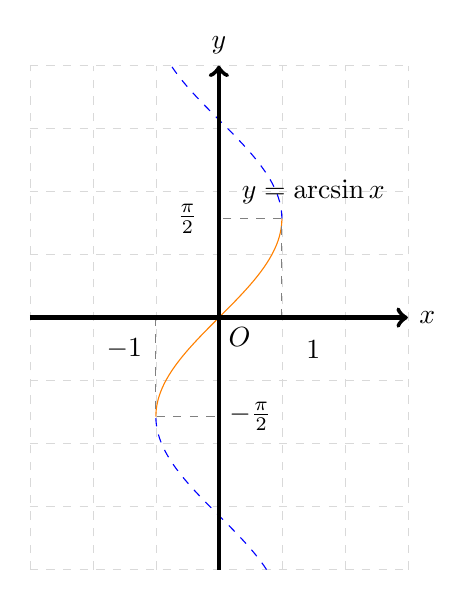
\begin{tikzpicture}[scale=\subscale]
		\draw[help lines, color=gray!30, dashed] (-3,-4) grid (3,4);

		\draw[color=blue,dashed]
			plot[domain=0.5*pi:4,samples=100] ({sin(\x r)},\x)
			plot[domain=-4:-0.5*pi,samples=100] ({sin(\x r)},\x);
		\draw[color=orange]
			plot[domain=-0.5*pi:0.5*pi,samples=100] ({sin(\x r)},\x)
			node[color=black] at (1.5,2) {\(y=\arcsin x\)};
		\draw [dashed,color=gray] (-1,0) -- (-1,-0.5*pi) -- (0,-0.5*pi)
			(1,0) -- (1,0.5*pi) -- (0,0.5*pi);

		\draw [->, ultra thick] (-3,0) -- (3,0) node[right]{\(x\)};
		\draw [->, ultra thick] (0,-4) -- (0,4) node[above]{\(y\)};

		\draw (-0.5,0.5*pi)node{\(\frac{\pi}{2}\)}
			(0.5,-0.5*pi)node{\(-\frac{\pi}{2}\)};
			\draw (0,0)node[below right]{\(O\)}
			(-1.5,-0.5)node{\(-1\)}
			(1.5,-0.5)node{\(1\)};
	\end{tikzpicture}
    \subcaption{反正弦函数}
    \end{subfigure}%
    \begin{subfigure}[b]{\subwidth}%
    \centering
	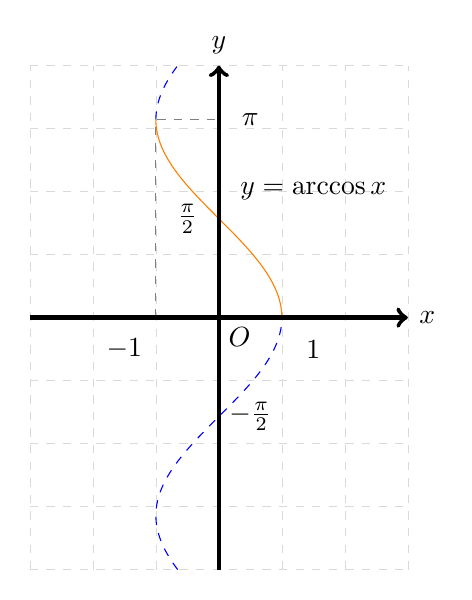
\begin{tikzpicture}[scale=\subscale]
		\draw[help lines, color=gray!30, dashed] (-3,-4) grid (3,4);

		\draw[color=blue,dashed]
			plot[domain=pi:4,samples=100] ({cos(\x r)},\x)
			plot[domain=-4:0,samples=100] ({cos(\x r)},\x);
		\draw[color=orange]
			plot[domain=0:pi,samples=100] ({cos(\x r)},\x)
			node[color=black] at (1.5,2) {\(y=\arccos x\)};
		\draw [dashed,color=gray] (-1,0) -- (-1,pi) -- (0,pi);

		\draw [->, ultra thick] (-3,0) -- (3,0) node[right]{\(x\)};
		\draw [->, ultra thick] (0,-4) -- (0,4) node[above]{\(y\)};

		\draw (-0.5,0.5*pi)node{\(\frac{\pi}{2}\)}
			(0.5,-0.5*pi)node{\(-\frac{\pi}{2}\)}
			(0.5,pi)node{\(\pi\)};
		\draw (0,0)node[below right]{\(O\)}
			(-1.5,-0.5)node{\(-1\)}
			(1.5,-0.5)node{\(1\)};
	\end{tikzpicture}
    \subcaption{反余弦函数}
    \end{subfigure}%

	\begin{subfigure}[b]{\linewidth}%
	\centering
	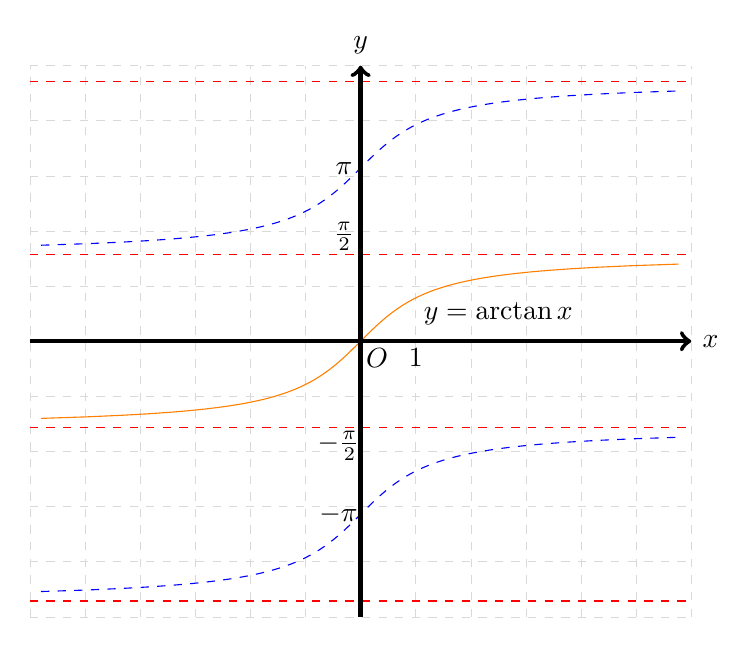
\begin{tikzpicture}[scale=.7]
		\draw[help lines, color=gray!30, dashed] (-6,-5) grid (6,5);

		\draw[color=red, dashed]
			(-6,-4.71237) -- (6,-4.71237)
			(-6,4.71237) -- (6,4.71237)
			(-6,-0.5*pi) -- (6,-0.5*pi)
			(-6,0.5*pi) -- (6,0.5*pi);
		\draw[color=blue, dashed]
			plot[domain=-1.4:1.4, samples=100] ({tan(\x r)},\x-pi)
			plot[domain=-1.4:1.4, samples=100] ({tan(\x r)},\x+pi);
		\draw[color=orange]
			plot[domain=-1.4:1.4, samples=100] ({tan(\x r)},\x);

		\draw [->, ultra thick] (-6,0) -- (6,0) node[right]{\(x\)};
		\draw [->, ultra thick] (0,-5) -- (0,5) node[above]{\(y\)};
		\draw (-0.3,1.9)node{\(\frac{\pi}{2}\)}
			(-0.4,-1.9)node{\(-\frac{\pi}{2}\)}
			(0.3,-0.3)node{\(O\)}
			(1,-0.3)node{\(1\)}
			(-0.3,pi)node{\(\pi\)}
			(-0.4,-pi)node{\(-\pi\)}
			(2.5,0.5)node{\(y=\arctan x\)};
	\end{tikzpicture}
	\subcaption{反正切函数}
	\end{subfigure}%
\caption{反三角函数的图形}
\label{figure:函数.反三角函数的图形}
\end{figure}

\subsubsection{反三角函数的性质}
\begin{theorem}[余角公式]
\begin{align}
\arcsin x + \arccos x &= \frac{\pi}{2}, \\
\arctan x + \arccot x &= \left\{ \begin{array}{cl}
\pi/2, & x > 0, \\
-\pi/2, & x < 0.
\end{array} \right.
\end{align}
\end{theorem}

\begin{theorem}[负数关系]
\begin{align}
\arcsin(-x) &= -\arcsin x, \\
\arccos(-x) &= \pi-\arccos x, \\
\arctan(-x) &= -\arctan x, \\
\arccot(-x) &= \pi-\arccot x, \\
\arcsec(-x) &= \pi-\arcsec x, \\
\arccsc(-x) &= -\arccsc x.
\end{align}
\end{theorem}

\begin{theorem}[倒数关系]
\begin{align}
\arcsin\frac{1}{x} &= \arccsc x, \\
\arccos\frac{1}{x} &= \arcsec x, \\
\arctan\frac{1}{x} &= \arccot x
	= \frac{\pi}{2} - \arctan x, \quad(x>0) \\
\arccot\frac{1}{x} &= \begin{cases}
	\arctan x, & x>0, \\
	\pi+\arctan x, & x<0,
	\end{cases} \\
\arccot\frac{1}{x} &= \left\{ \def\arraystretch{1.5} \begin{array}{lc}
	\frac{\pi}{2} - \arccot x, & x>0, \\
	\frac{3\pi}{2} - \arccot x, & x<0,
	\end{array} \right. \\
\arcsec\frac{1}{x} &= \arccos x, \\
\arccsc\frac{1}{x} &= \arcsin x.
\end{align}
\end{theorem}

\begin{theorem}[三角关系]
\begin{align}
\sin(\arcsin{x}) &= x, \\
\cos(\arccos{x}) &= x, \\
\tan(\arctan{x}) &= x, \\
\arcsin(\sin x) &= x, \quad x \in (-\frac{\pi}{2},\frac{\pi}{2}), \\
\arccos(\cos x) &= x, \quad x \in (0,\pi), \\
\arctan(\tan x) &= x, \quad x \in (-\frac{\pi}{2},\frac{\pi}{2}), \\
\sin(\arccos{x}) = \cos(\arcsin{x}) &= \sqrt{1 - x^2}, \\
\tan(\arccot{x}) = \cot(\arccot{x}) &= \frac{1}{x}, \\
\sin(\arctan{x}) = \cos(\arccot{x}) &= \frac{x}{\sqrt{1+x^2}}, \\
\cos(\arctan{x}) = \sin(\arccot{x}) &= \frac{1}{\sqrt{1+x^2}}.
\end{align}
\end{theorem}

\begin{theorem}[和差公式]
\begin{align}
&\hspace{-10pt}
\arcsin x + \arcsin y \\
	&= \arcsin(x \sqrt{1-y^2} + y \sqrt{1-x^2}),
		\quad(xy\leqslant0 \lor x^2+y^2\leqslant1) \\
	&= \pi - \arcsin(x \sqrt{1-y^2} + y \sqrt{1-x^2}),
		\quad(x>0, y>0, x^2+y^2>1) \\
	&= -\pi - \arcsin(x \sqrt{1-y^2} + y \sqrt{1-x^2}),
		\quad(x<0, y<0, x^2+y^2>1) \\
&\hspace{-10pt}
\arcsin x - \arcsin y \\
	&= \arcsin(x \sqrt{1-y^2} - y \sqrt{1-x^2}),
		\quad(xy\geqslant0 \lor x^2+y^2\leqslant1) \\
	&= \pi - \arcsin(x \sqrt{1-y^2} - y \sqrt{1-x^2}),
		\quad(x>0, y<0, x^2+y^2>1) \\
	&= -\pi - \arcsin(x \sqrt{1-y^2} + y \sqrt{1-x^2}),
		\quad(x<0, y>0, x^2+y^2>1) \\
&\hspace{-10pt}
\arccos x + \arccos y \\
	&= \arccos[xy - \sqrt{(1-x^2)(1-y^2)}],
		\quad(x+y\geqslant0) \\
	&= 2\pi - \arccos[xy - \sqrt{(1-x^2)(1-y^2)}],
		\quad(x+y<0) \\
&\hspace{-10pt}
\arccos x - \arccos y \\
	&= -\arccos[xy + \sqrt{(1-x^2)(1-y^2)}],
		\quad(x \geqslant y) \\
	&= \arccos[xy + \sqrt{(1-x^2)(1-y^2)}],
		\quad(x<y) \\
&\hspace{-10pt}
\arctan x + \arctan y \\
	&= \arctan\frac{x+y}{1-xy},
		\quad(xy<1) \\
	&= \pi+\arctan\frac{x+y}{1-xy},
		\quad(x>0,xy>1) \\
	&= -\pi+\arctan\frac{x+y}{1-xy},
		\quad(x<0,xy>1) \\
&\hspace{-10pt}
\arctan x - \arctan y \\
	&= \arctan\frac{x-y}{1+xy},
		\quad(xy>-1) \\
	&= \pi+\arctan\frac{x-y}{1+xy},
		\quad(x>0,xy<-1) \\
	&= -\pi+\arctan\frac{x-y}{1+xy},
		\quad(x<0,xy<-1)
\end{align}
\end{theorem}

\begin{figure}
\centering
\begin{tikzpicture}
  \draw[help lines, color=gray!30, dashed] (0,0) grid (4,3);
  \coordinate (A) at (0,0);
  \coordinate (B) at (4,0);
  \coordinate (C) at (4,3);
  \draw (A)node[left]{\(A\)} -- (B)node[right]{\(B\)}node[midway,below]{\(1\)} -- (C)node[right]{\(C\)}node[midway,right]{\(x\)} -- (A)node[midway,above left]{\(\sqrt{1+x^2}\)} pic["\(\theta\)",draw=orange,-,angle eccentricity=2,angle radius=0.3cm]{angle=B--A--C} pic[draw=gray,-,angle radius=0.3cm]{right angle=C--B--A};
  \draw (5,1.5)node[right]{\(\begin{aligned}
  &\tan\theta = x \implies \theta = \arctan x, \\
  &\cos\theta = \cos(\arctan x) = \frac{1}{\sqrt{1+x^2}}, \\
  &\sin\theta = \sin(\arctan x) = \frac{x}{\sqrt{1+x^2}}, \\
  &\cot\theta = \cot(\arctan x) = \frac{1}{x}.
  \end{aligned}\)};
\end{tikzpicture}
\caption{三角函数与反三角函数之间的联系}
\end{figure}

\subsection{双曲函数、反双曲函数}
\begin{definition}[双曲函数]
\begin{align}
\sinh{x} &\defeq \frac{e^x - e^{-x}}{2}, \\
\cosh{x} &\defeq \frac{e^x + e^{-x}}{2}, \\
\tanh{x} &\defeq \frac{\sinh x}{\cosh x} = \frac{e^x - e^{-x}}{e^x + e^{-x}}, \\
\coth{x} &\defeq \frac{1}{\tanh{x}} = \frac{e^x + e^{-x}}{e^x - e^{-x}},
\end{align}
其中,%
\(\sinh{x}\)被称为\textbf{双曲正弦},%
\(\cosh{x}\)被称为\textbf{双曲余弦},%
\(\tanh{x}\)被称为\textbf{双曲正切},%
\(\coth{x}\)被称为\textbf{双曲余切}.
\end{definition}

\begin{definition}[反双曲函数]
\begin{align}
\arsh{x} &= \ln(x + \sqrt{x^2 + 1}), &x \in (-\infty,+\infty) \\
\arch{x} &= \ln(x - \sqrt{x^2 - 1}), &x \in [1,+\infty) \\
\arth{x} &= \frac{1}{2} \ln\frac{1 + x}{1 - x}, &x \in (-1,1) \\
\arcth{x} &= \frac{1}{2} \ln\frac{x + 1}{x - 1}, &x \in (-\infty,-1) \cup (1,+\infty)
\end{align}
其中,%
\(\arsh{x}\)被称为\textbf{反双曲正弦},%
\(\arch{x}\)被称为\textbf{反双曲余弦},%
\(\arth{x}\)被称为\textbf{反双曲正切},%
\(\arcth{x}\)被称为\textbf{反双曲余切}.
\end{definition}

\begin{property}
\(\sinh x\)是奇函数,即对\(\forall x \in [-a,a]\)有\[
\sinh(-x) = -\sinh x;
\]

\(\cosh x\)是偶函数,即对\(\forall x \in [-a,a]\)有\[
\cosh(-x) = \cosh x.
\]
\end{property}

\begin{property}
\(\cosh{x}\)有下界:\[
\cosh{x} \geqslant 1
\]当且仅当\(x=0\)时,上式取等号.
\end{property}

\begin{theorem}
\begin{gather}
\sinh(x \pm y) = \sinh{x}\cosh{y} \pm \cosh{x}\sinh{y} \\
\cosh(x \pm y) = \cosh{x}\cosh{y} \pm \sinh{x}\sinh{y} \\
\tanh(x + y) = \frac{\tanh{x} + \tanh{y}}{1 + \tanh{x}\tanh{y}}
\end{gather}
\begin{proof}
根据双曲函数的定义有
\begin{align*}
\sinh{x}\cosh{y}+\cosh{x}\sinh{y}
&= \frac{e^x - e^{-x}}{2} \frac{e^y + e^{-y}}{2} + \frac{e^x + e^{-x}}{2} \frac{e^y - e^{-y}}{2} \\
&= \frac{1}{4} (e^x e^y + e^x e^{-y} - e^{-x} e^y - e^{-x} e^{-y} \\
&\qquad+ e^x e^y - e^x e^{-y} + e^{-x} e^y - e^{-x} e^{-y}) \\
&= \frac{1}{4} (2 e^x e^y - 2 e^{-x} e^{-y}) \\
&= \frac{1}{2} (e^{x+y} - e^{-x-y}) = \sinh(x+y).
\end{align*}

\begin{align*}
\cosh{x}\cosh{y}+\sinh{x}\sinh{y}
&= \frac{e^x + e^{-1}}{2} \frac{e^y + e^{-y}}{2} + \frac{e^x - e^{-x}}{2} \frac{e^y - e^{-y}}{2} \\
&= \frac{1}{4} (e^x e^y + e^x e^{-y} + e^{-x} e^y + e^{-x} e^{-y} \\
&\qquad+ e^x e^y - e^x e^{-y} - e^{-x} e^y + e^{-x} e^{-y}) \\
&= \frac{1}{4} (2 e^x e^y + 2 e^{-x} e^{-y}) \\
&= \frac{1}{2} (e^{x+y} + e^{-x-y}) = \cosh(x+y).
\qedhere
\end{align*}
\end{proof}
\end{theorem}

\begin{theorem}
\begin{gather}
\cosh^2{x} - \sinh^2{x} = 1 \\
\sinh{x} + \cosh{x} = e^x \\
\cosh{x} - \sinh{x} = e^{-x} \\
1 - \tanh^2{x} = \frac{1}{\cosh^2{x}} \\
\coth^2{x} - 1 = \frac{1}{\sinh^2{x}}
\end{gather}
\begin{proof}
根据双曲函数的定义有
\begin{align*}
\cosh^2{x}-\sinh^2{x}
&=\left(\frac{e^x + e^{-x}}{2}\right)^2-\left(\frac{e^x - e^{-x}}{2}\right)^2 \\
&=\frac{e^{2x}+2+e^{-2x}}{4}-\frac{e^{2x}-2+e^{-2x}}{4}
=1. \qedhere
\end{align*}
\end{proof}
\end{theorem}

\begin{theorem}
\begin{gather}
\sinh{2x} = 2 \sinh{x}\cosh{x} \\
\cosh{2x} = \cosh^2{x} + \sinh^2{x}
\end{gather}
\end{theorem}

\subsection{幂指函数}
\begin{definition}
形如\[
y = u(x)^{v(x)},
\quad u(x) > 0 \land u(x) \not\equiv 1
\]的函数称为\textbf{幂指函数}.
\end{definition}
值得注意的是,幂指函数不是初等函数.

\section{抽象函数}
方程\[
f(x+y) = f(x) + f(y) + c \quad(c\text{是常数})
\]确定的函数\(f\)称为直线型抽象函数.

方程\[
f(xy) = f(x) f(y)
\]确定的函数\(f\)称为幂函数型抽象函数.

方程\[
f(x+y) = f(x) f(y)
\]或\[
f(xy) = [f(x)]^y
\]确定的函数\(f\)称为指数函数型抽象函数.

方程\[
f(xy) = f(x) + f(y)
\]或\[
f\left(\frac{x}{y}\right) = f(x) - f(y)
\]确定的函数\(f\)称为对数函数型抽象函数.

方程\[
f(x) + f(y) = 2 f\left(\frac{x+y}{2}\right) f\left(\frac{x-y}{2}\right)
\]或\[
f(x+y) = \frac{f(x) + f(y)}{1 - f(x) f(y)}
\]确定的函数\(f\)称为三角函数型抽象函数.

\section{初等函数}
\begin{definition}
\emph{常函数}、\emph{幂函数}、\emph{指数函数}、\emph{对数函数}、\emph{三角函数}、\emph{反三角函数}这六类函数统称为\textbf{基本初等函数}.
由常数和基本初等函数经过有限次四则运算和有限次函数复合步骤所构成并可用一个式子表示的函数,称为\textbf{初等函数}.
\end{definition}
